% Airborne ice-penetrating radar data has been used to explore past ice sheet evolution and flow as well as to indirectly probe modern ice sheet boundary conditions. In order to do so, it is useful to determine the age of radar-observed englacial layers to provide constraints on the timing of features indicative of  change within the ice. More than a dozen surveys over the last several decades have provided extensive coverage of central West Antarctica, including the Thwaites Glacier catchment and Marie Byrd Land regions. These surveys pass near the Byrd (80.0167$^\circ$S, 119.5167$^\circ$W) and WAIS Divide (79.48$^{\circ}$S, 112.11$^{\circ}$W) ice cores, making it possible to correlate ice core chronologies with observed englacial layers at depth. 

% The WAIS Divide ice core has been dated to 68 ka and the Byrd ice core has been dated to 91 ka, thus providing the potential for dating West Antarctic englacial ice through most of the Last Interglacial cycle. However, while a robust age-depth chronology is available for the recently-drilled WAIS Divide ice core, the Byrd ice core chronology -- the first deep core to be drilled in Antarctica -- lacks sufficient error analysis. We derive uncertainty for the Byrd ice core chronology using a combination of ice flow modeling and correlation of layers traced between the well-dated WAIS Divide ice core and the Byrd ice core. Additionally, the contribution of uncertainty in layer depth observed from ice-penetrating radar has not been computed for the West Antarctic. Using specifications of the radar system, we quantify radar depth uncertainty and include it when assigning ages to radar-observed layers of interest.

% Age registration of englacial layers is most practical for layers which can be tracked continually both to an ice core and throughout a large domain. We identify 9 such layers at the WAIS Divide ice core and 10 layers at the Byrd ice core which are dated and tracked for hundreds of line-km in central West Antarctica. The result is isochronous surfaces which reveal evidence of deformation in the ice sheet and could identify areas of changes in accumulation, flow, or subglacial boundary conditions. This three-dimensional view of the inside of the West Antarctic ice sheet provides a new avenue to validate ice sheet models and explore past behavior and dynamics of the ice sheet. 

% \begin{figure}[!h]
% %\begin{center}
% \centering
% 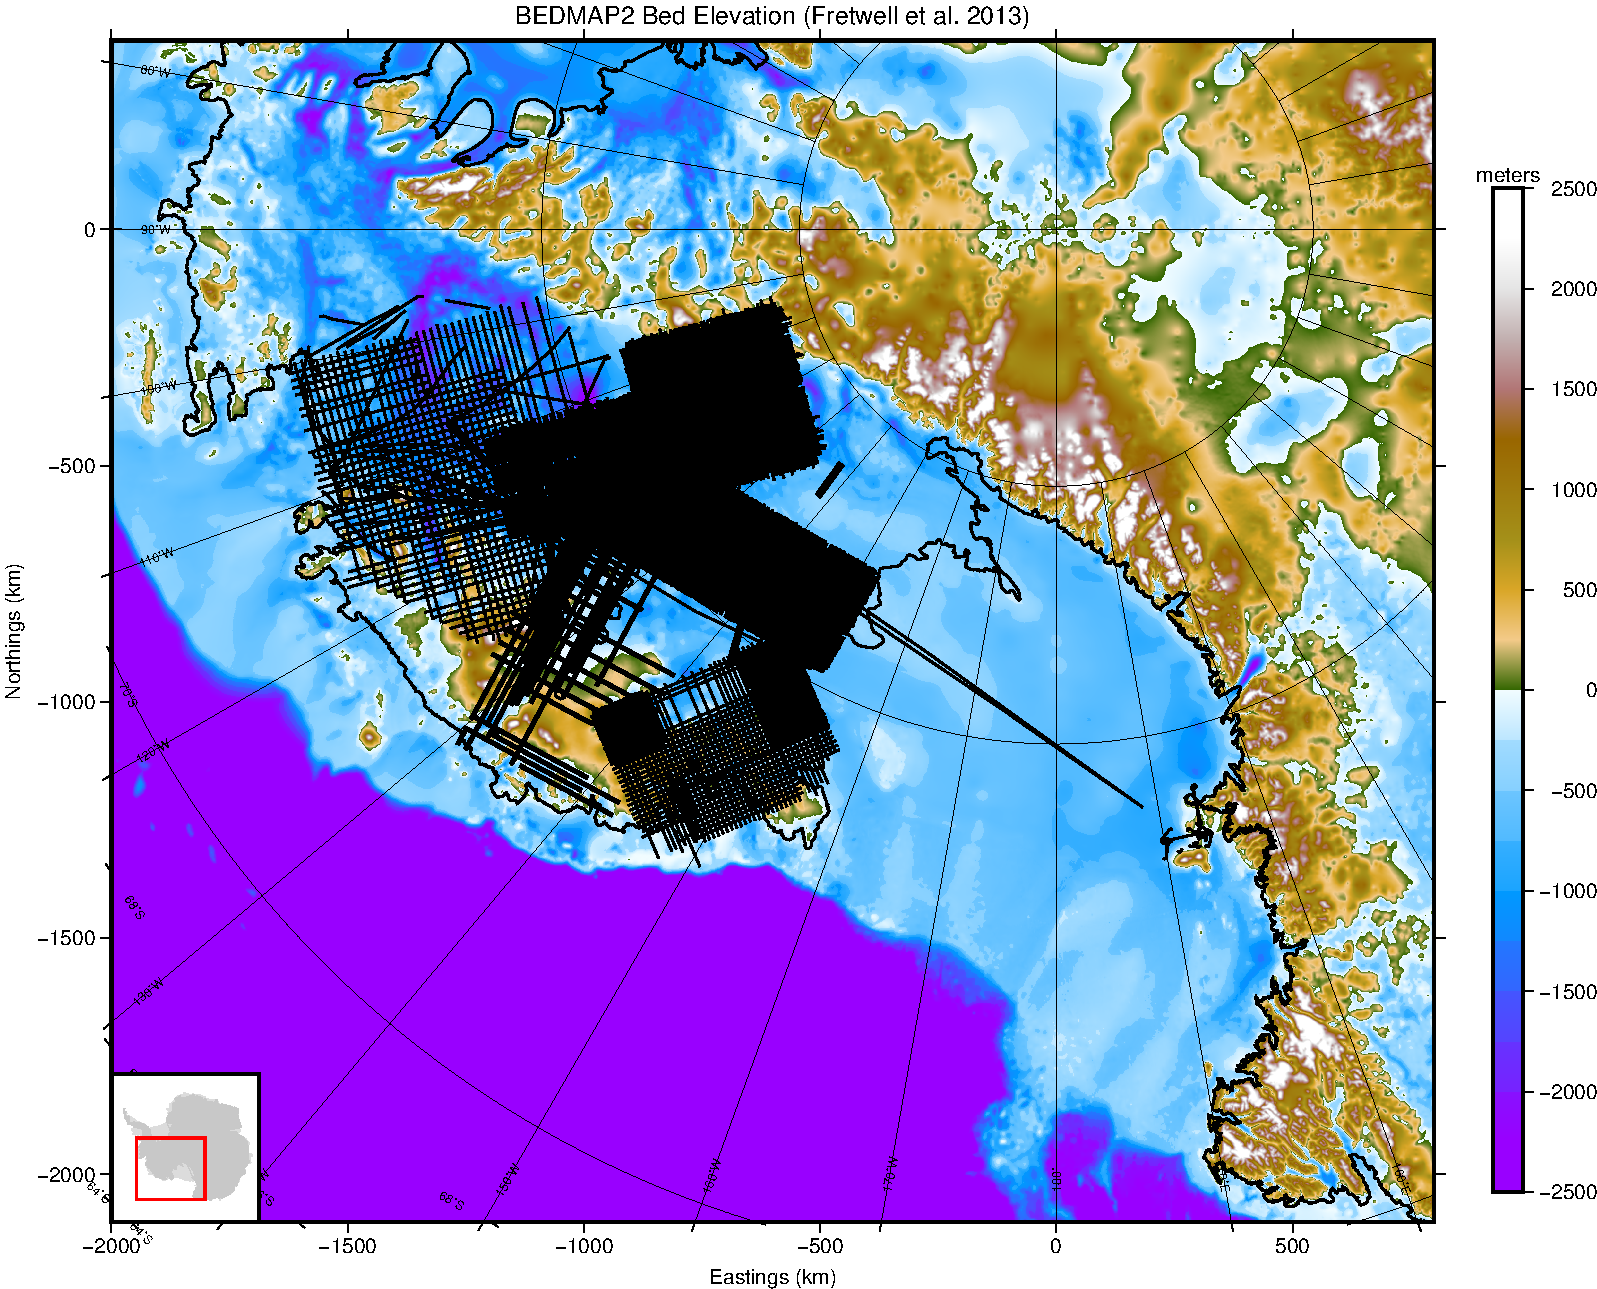
\includegraphics[scale=0.3]{figures/Fig1_WAISall_bed2}
% %\captionsetup{width=.9\textwidth}
% \caption[]{Map of central West Antarctic with available airborne geophysical radar surveys (black lines) and (\textbf{will be updated to have:} WAIS Divide and Byrd ice core locations (blue triangles) overlain. Gray shading is surface elevation according to Fretwell et al. 2013. }
% %\end{center}
% \label{fig:radarmap}
% \end{figure}

% Start version from 2 Aug 2017%
%The Byrd ice core (80.0167$^\circ$S, 119.5167$^\circ$W) was the first to be drilled to bedrock in Antarctica \citep{gow1968}. The proximity of the core to fast-changing ice of both the Siple and Amundsen Sea coasts in West Antarctica makes it a potentially important source of information in studies of the response of the West Antarctic Ice Sheet (WAIS) to changing climatic conditions. More than three extensive radar surveys pass near the core site, including the recent GIMBLE survey filling a data coverage gap in Marie Byrd Land \citep{duncan}, make it particularly useful for dating paleo ice dynamics observed in the central WAIS. Dated englacial radar data enables information from the entire ice volume--rather than only surface observations--to constrain ice dynamics in the central WAIS, including the Thwaites Glacier catchment and Marie Byrd Land.

%While the Byrd ice core has been dated to more than 90ka \citep{}, nearly back to the Last Interglacial, the chronology lacks estimates of uncertainty in age and depth. Here we use a Bayesian technique to compute a probabilistic chronology for the Byrd ice core which is constrained by existing ice core chronology results. This method inverts for probability distributions of ice sheet parameter values consistent with the recorded ice core chronology. 

%We use the modeled chronology to assign ages to englacial reflectors traced through the central WAIS. These reflectors encode information about ice sheet boundary conditions and paleo ice dynamics \citep[e.g.][]{}. They are the result of dielectric contrasts in the ice due to variations in composition, crystal fabric, temperature, and other ice properties. Each continuous reflector is assumed to be the result of a distinct surface deposition episode with a distinguishable dielectric signature and is therefore assumed to be isochronous \citep{fujita2000}. 

%The isochronous nature of englacial reflectors implies that assigning an age to each reflector at the Byrd ice core site effectively dates the reflector anywhere it can be continuously traced in the region. This allows for extensive age registration throughout the ice column and radar survey domain and also for validation of our results at the Byrd ice core with the recently-drilled WAIS Divide ice core chronology, as has been done in East Antarctica \citep{cavitte2016}. The WAIS Divide ice core (79.48$^{\circ}$S, 112.11$^{\circ}$W) provides an ice chronology with uncertainty quantification as far as back as 67ka \citep[][C. Buizert, personal communication]{buizert2015} and is therefore an independent validation of our improved Byrd ice core chronology. 

%Having two ice cores from which to date englacial reflectors enables more extensive dating, particularly in areas of complicated basal topography where the radar isochrones experience increased discontinuity and cannot be tracked for long distances. This is the case near the Marie Byrd Land icecap, for example, where reflectors present at the Byrd ice core site have been traced around areas of disruption due to high-relief bed terrain. In general, deeper reflectors are more difficult to track extensively in the WAIS due to lower reflection amplitudes and increased disruption. However, we interpolate three-dimensional isochronous surfaces for the extent of each of four observed reflectors which sample the ice depth. The modeled chronology is used to assign ages to these surfaces.

%End version from 2 Aug 2017%

Isochronous, englacial radar reflectors observed by ice-penetrating radar record the depth and extent of isosurfaces with shared physical properties \citep{siegert1998,dowdeswell2004}. These reflectors can map the age structure of an ice sheet, with the thickness of layers bounded by reflectors revealing information about ice flow dynamics and variable ice properties. Such observations have been used in Greenland and Antarctica to infer the ice flow history of the ice sheets in response to changing climate regimes in the past \citep{macgregor2015}. To provide such historical climatic context, reflectors are assigned ages by correlation to a known chronology, such as at an ice core site \citep{cavitte2016}. Dating englacial reflectors enables information from the entire ice volume, not only surface observations, to constrain ice sheet dynamics. However, combining information from ice cores and radar observations is intrinsically complicated by the fact that ice core chronologies assign discrete ages to samples of ice, while radar reflectors track packets of ice with finite thickness that span a range of ages, particularly at depth where age is more sensitive to depth due to shear thinning of the ice. 

To understand how well radar reflectors can be dated, we use Bayesian methods %\citep{metropolis1953,hastings1970,gelfand1992} 
to synthesize information from ice cores, radar sampling, ice flow modeling, and our knowledge of the leading sources of uncertainty within the radar and ice core data sources. We apply our approach to the central West Antarctic Ice Sheet (WAIS), an area containing the potential for unforced retreat where ice dynamics are of particular interest for projections of future sea level rise. In addition to being of scientific importance, the central WAIS is an area with concentrated radar surveys and two deep ice cores, the Byrd ice core \citep{gow1968} and the WAIS Divide ice core \citep{buizert2015}. In particular, the proximity of the Byrd ice core (80.0167$^\circ$S, 119.5167$^\circ$W) to fast-changing ice of both the Siple and Amundsen Sea coasts in West Antarctica makes it a potentially important source of information about the response of the WAIS to climate change.
%In particular, the proximity of the Byrd ice core \cite[(80.0167$^\circ$S, 119.5167$^\circ$W),][]{gow1968} to fast-changing ice of both the Siple and Amundsen Sea coasts in West Antarctica makes it a potentially important source of information in studies of the response of the West Antarctic Ice Sheet (WAIS) to changing climatic conditions.

The Byrd ice core is co-located with several extensive radar surveys (Figure~\ref{fig:radarmap}) and contains an ice record that extend back to more than 90 ka \citep{blunier2001}, nearly back to the Last Interglacial. Rather than use existing chronologies for the age-depth relationship at the Byrd ice core, which do not sufficiently characterize its uncertainty, we generate our own chronologies using Bayesian strategies to synthesize an ice flow model with age-depth data obtained from volcanics sampled from the Byrd ice core \citep{gow1968,gow1970,hammer1997}. This method allows us to simulate the co-dependence in dating errors within and between different radar reflectors.

The four reflectors in this study were chosen as a representative sample of the ice column and for their signal-to-noise ratio and continuity. It is possible to use this method to date additional englacial reflectors observed using radar in this area, but the usefulness of such ages extend only as far as the isochronous reflectors can be horizontally traced. While this method is less helpful for dating discontinuous reflectors, it could inform relative ages for sections of discontinuous reflectors adjacent to dated reflectors in the ice column  \citep[e.g.][]{macgregor2015}.

%However, there are currently no formal estimates of uncertainty in its chronology. Quantifying such uncertainty is challenging because it arises from a number of sources, including measured depth and age of the ice and unknown local ice flow parameters. This problem is nontrivial because age-depth solutions are nonunique and depend on solutions elsewhere in the ice column. Despite this, it is important to include uncertainty in the Byrd ice core chronology when using it to characterize the englacial age structure of the greater WAIS to limit the propagation of unrealistic certainty in age, particularly at depth where shear thinning is dominant and uncertainties are expected to be greatest. 

We consider two quantities of interest in this problem: radar-inferred depths from observed two-way travel time (TWTT) and dated volcanics from the Byrd ice core. The primary sources of uncertainty in radar depths include the speed of electromagnetic radiation in ice, the density and thickness of the firn layer, and radar range precision. The error on range precision is determined independently for each reflector and the ice surface, while errors in velocity and firn are systematic (common) across all reflectors of interest in the ice column which are deeper than the firn layer. To estimate the ages of reflectors, we make use of dates determined for volcanic markers in the ice column \citep{hammer1997}. %However, we must estimate age errors in the absence of published uncertainty on the volcanic record. 
In the absence of published uncertainty in the volcanic record, we use a Bayesian strategy to include an uncertain age uncertainty.
An ice flow model is used to smoothly transfer information from the volcanics to the estimated depth of our reflectors of interest. To do so, it is necessary to infer flow physics parameters and accumulation rate history. Estimated ice flow and accumulation rate parameters are dependent on one another and on depth and are applied to the full ice column. A Bayesian framework allows us to describe all  components of the problem within a single calculation, but requires stochastic sampling to estimate the marginal probability of reflector depth (and therefore age) as a function of observed TWTT and volcanics.



%We use a novel approach to probabilistically date englacial radar reflectors observed near the Byrd ice core given information about the radar-observed two-way travel time (TWTT), previously-computed age-depth observations of the ice core, constraints on englacial stratigraphy, and other factors. A simple flow model is used to show how age of the reflectors varies with depth, taking into account our knowledge of ice flow physics and surface accumulation rate. While some information about these parameters is known, large uncertainties remain. To account for these uncertainties and nonunique solutions of the age-depth chronology, we use a probabilistic method to estimate uncertainty in the parameter values to find combinations of parameter values which lead to age-depth solutions consistent with observations.



%The estimated Byrd ice core chronology and published WAIS Divide ice core record are used to assign dates to englacial radar reflectors observed at the ice core sites, which are assumed isochronous \citep{cite}. These isochronous reflectors have been traced extensively throughout Central West Antarctica. As such, we leverage the ice core chronologies to date observable ice stratigraphy hundreds of kilometers from existing ice core records.


Section~\ref{byrdchronology} discusses the formulation of the Bayesian problem and methods for finding solutions of the age and depth of observed englacial radar reflectors. Section~\ref{agedepthresults} shows results for the probability distributions of reflector age and depth as well as a comparison to the WAIS Divide ice core chronology as an independent check on our results. %Section~\ref{layersurfaces} explores the application of ages at the ice cores to extensive isochronous surfaces throughout West Antarctica, which can be used to analyze paleo flow and boundary conditions in the region. 
We also calculate an error budget to determine the dominant contributions to age-depth uncertainty, discussed in Section~\ref{discussion}.
